\chapter{Finanzierung}
\section{Zentrale Annahmen}
\begin{itemize}
	\item Förderungen/Zuschüsse sind nicht in den Berechnungen enthalten
	\item Keine Gewinnausschüttung bzw. Bonifikationen an die Unternehmensgründer
	\item Zahlungsziele (Kunden und Lieferanten): 30 Tage
\end{itemize}

\section{Finanzierungsmodell}
Die Finanzierung des Unternehmen erfolgt durch 4 Säulen. 

\noindent
\begin{tabular}{@{}>{\raggedright\arraybackslash}p{1.8cm}@{}>{\raggedright\arraybackslash}p{\textwidth - 1.8cm}}
 
	\textbf{Säule 1:} & Der Hersteller des Roboters finanziert die Anpassung des System an den jeweiligen Roboter mit der Entwicklungsgebühr. \\ 

	\textbf{Säule 2:} & Die Verwendung des Systems ist lizenziert. Für jeden Roboter, in dem das System zum Einsatz kommt, ist eine jährliche Lizenzgebühr fällig. Diese ist abhängig davon, wie viel Einsparungspotential durch das System möglich ist und welche Version des Systems verwendet wird. \\
	
	\textbf{Säule 3:} & Der Roboterhersteller finanziert eine Weiterentwicklung eines bestehenden Systems. \\
	
	\textbf{Säule 4:} & Damit der Betreiber das System verwenden müssen seine Mitarbeiter geschult werden.
\end{tabular}

\subsection{Entwicklungsgebühr}
\subsubsection{Neuentwicklung}
Die Entwicklungsgebühr ist unabhängig vom Roboter und Hersteller. Sie stützt sich darauf, dass der Roboter für die Betreiber attraktiver wird, da dieser eine jährliche Stromersparnis und dadurch resultierende Kostenersparnis mit sich bringt.\\
Die Entwicklungsgebühr beträgt $100.000,00$\officialeuro.\\
Diese kann um bis zu $20$\% verringert werden sofern entsprechende Gegenleistungen angeboten werden.

\subsubsection{Weiterentwicklung}
Das grundlegende System unterliegt einer ständigen Weiterentwicklung. Neue Versionen des System müssen jedoch wieder an einen Roboter angepasst werden. Abhängig von den Versionsunterschieden beträgt die Gebühr zwischen $25.000$ und $50.000$\officialeuro.\\
Diese kann um bis zu $20$\% verringert werden sofern entsprechende Gegenleistungen angeboten werden.

\subsection{Lizenzgebühren}
Die Verwendung des Systems verschafft dem Betreiber einen enormen Wettbewerbsvorteil. Damit der Betreiber das System verwenden kann ist eine jährliche Lizenzgebühr fällig. Diese beträgt für die \textit{Version 1} mindestens $500,00$\officialeuro. Ab $5,00$\% steigt die Lizenzgebühr proportional zur Energieersparnis. Als zweiter Referenzpunkt gilt die $30,00$\%-Marke bei der die Lizenzgebühr $2.000,00$\officialeuro~beträgt, siehe Abbildung \ref{fig:lizenzgebuehr}.
\begin{figure}[h]
	\centering
	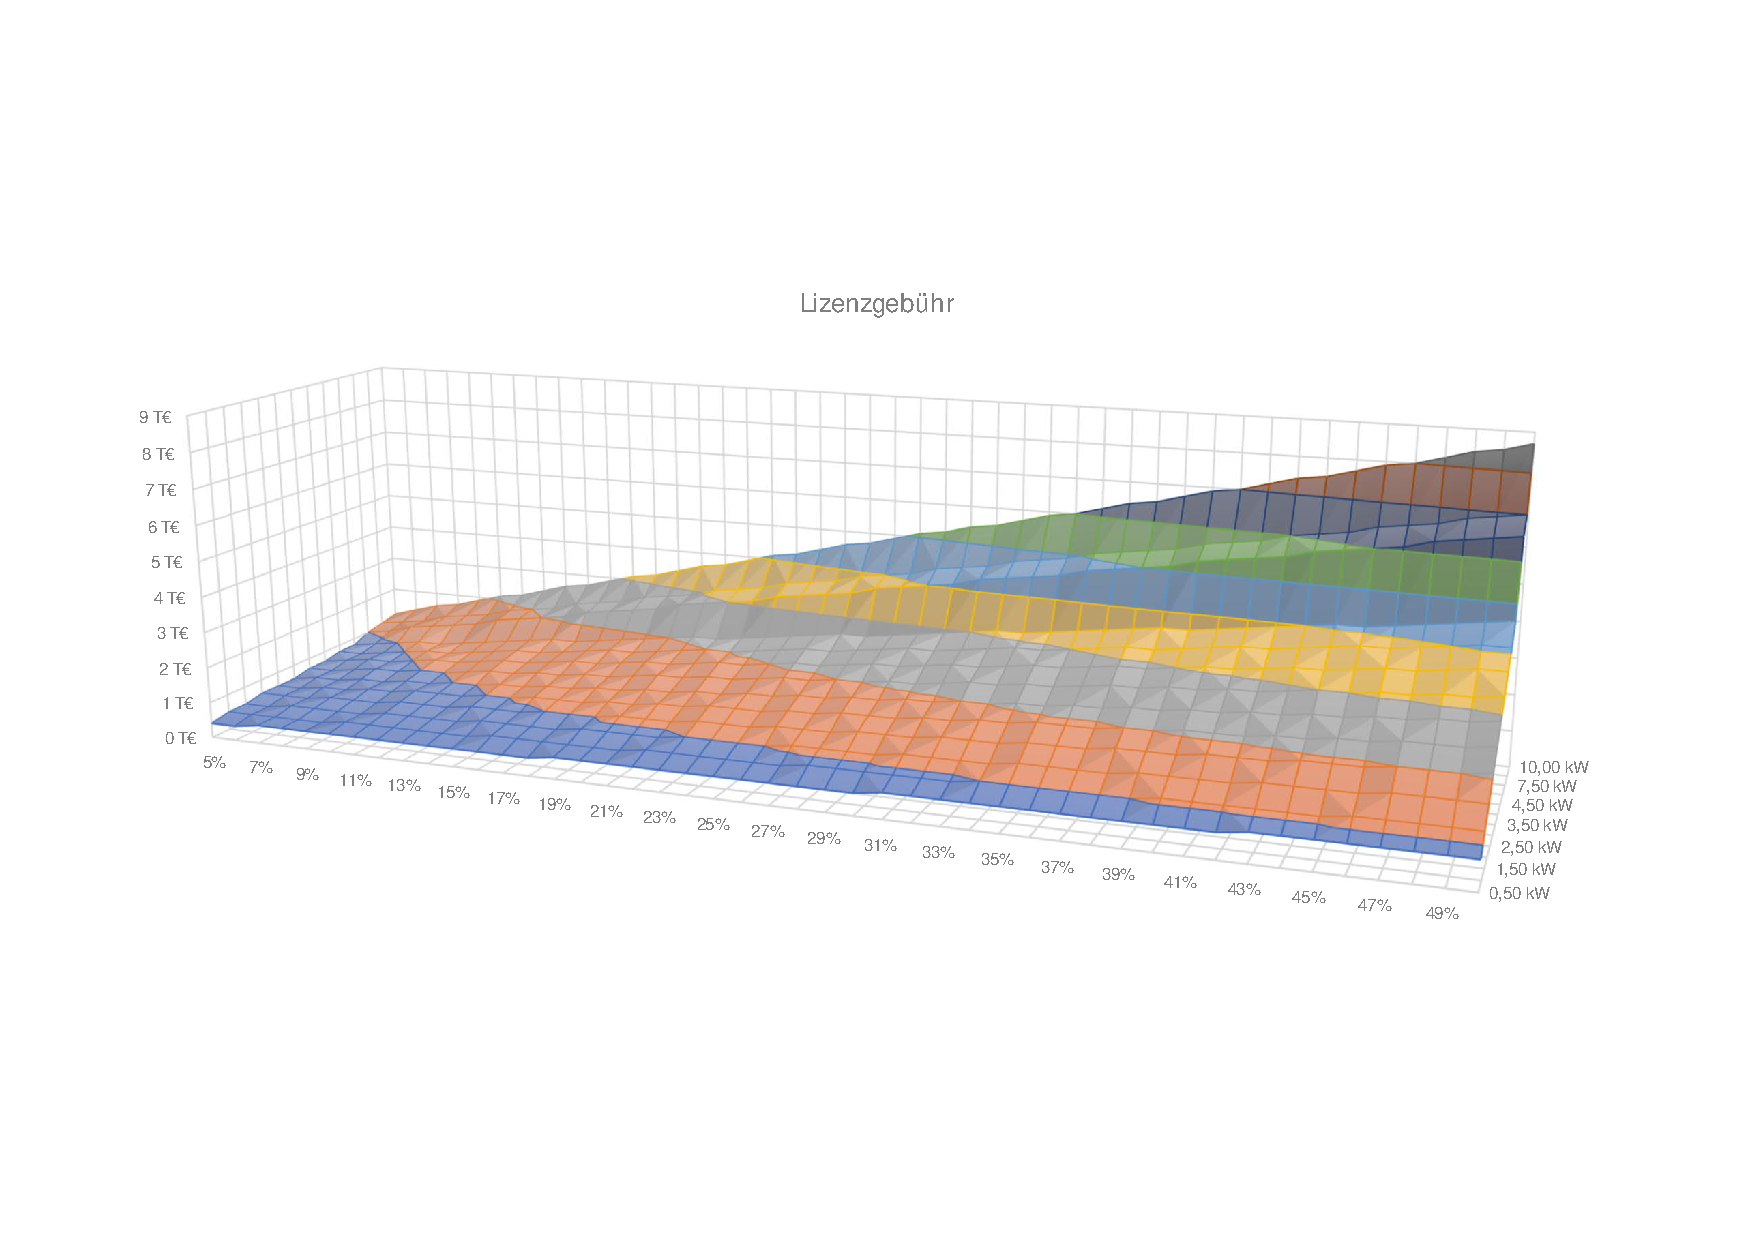
\includegraphics[width=10cm]{Lizenzgebuehr.pdf}
	\caption{Lizenzgebühr für die \textit{Version 1}}
	\label{fig:lizenzgebuehr}
\end{figure}

\paragraph*{Versionsupdate:}
Wir eine neue Version des Systems veröffentlicht, kann sich die Lizenzgebühr verändern. Die Unterstützung von mehreren Versionen des System und den dazugehörigen Lizenzgebührmodellen ist möglich.

\subsection{Schulung}
\subsubsection{Grundschulung}
Die Grundschulung umfasst die Installation und Verwendung des System mit der Robotersteuerung. Die Schulung dauert 2 Tage und die Kosten betragen $800,00$\officialeuro~pro Person.

\subsubsection{Intensivschulung}
Im System können Parameter verändert werden um mögliche spezielle Anforderungen abdecken zu können. Wie die Parameter verändert werden können und welche Auswirkung die Veränderungen haben ist Teil der Intensivschulung. Diese dauert 3 Tage und die Kosten betragen $1.500,00$\officialeuro~pro Person.

\section{Basis-Scenario}
Für das Basis-Scenario wurden folgende Annahmen getroffen:
\begin{itemize}
	\item Es werden in den folgenden 4 Jahren 20 Neuentwicklungen in Auftrag gegeben (Aufteilung:~3/5/6/6). Damit werden $~12$\% der Robotertypen der 5 wichtigsten Hersteller mit dem System ausgerüstet, siehe Kapitel \ref{sec:Marketing}.
	\item Die Lizenzvergabe verteilt sich wie folgt:\newline (Angaben in Prozent vom weltweitem Absatz von Industrierobotern ($400.000$ Stück), siehe Kapitel \ref{sec:Marketing})
	\begin{itemize}
		\item 1. Jahr: $0,00$\% (0 Roboter)
		\item 2. Jahr: $0,03$\% (~120 Roboter)
		\item 3. Jahr: $0,09$\% (~360 Roboter)
		\item 4. Jahr: $0,25$\% (~1000 Roboter)
	\end{itemize}
	\item Die durchschnittlichen Lizenzkosten betragen $1.500,00$\officialeuro.
	\item Es wird mit 60 Teilnehmer an der Grundschulung innerhalb der nächsten 4 Jahren gerechnet (Aufteilung:~8/12/16/24). Zusätzlich nehmen 10 Teilnehmer die Intensivschulung in Anspruch (Aufteilung: 0/2/3/5).
\end{itemize}

\subsection{Break-Even-Point}
Der BEP wird im Basis-Szenario im 3. Jahr erreicht, siehe Abbildung \ref{fig:BasisSzenario-BEP}.
\begin{figure}[h]
	\centering
	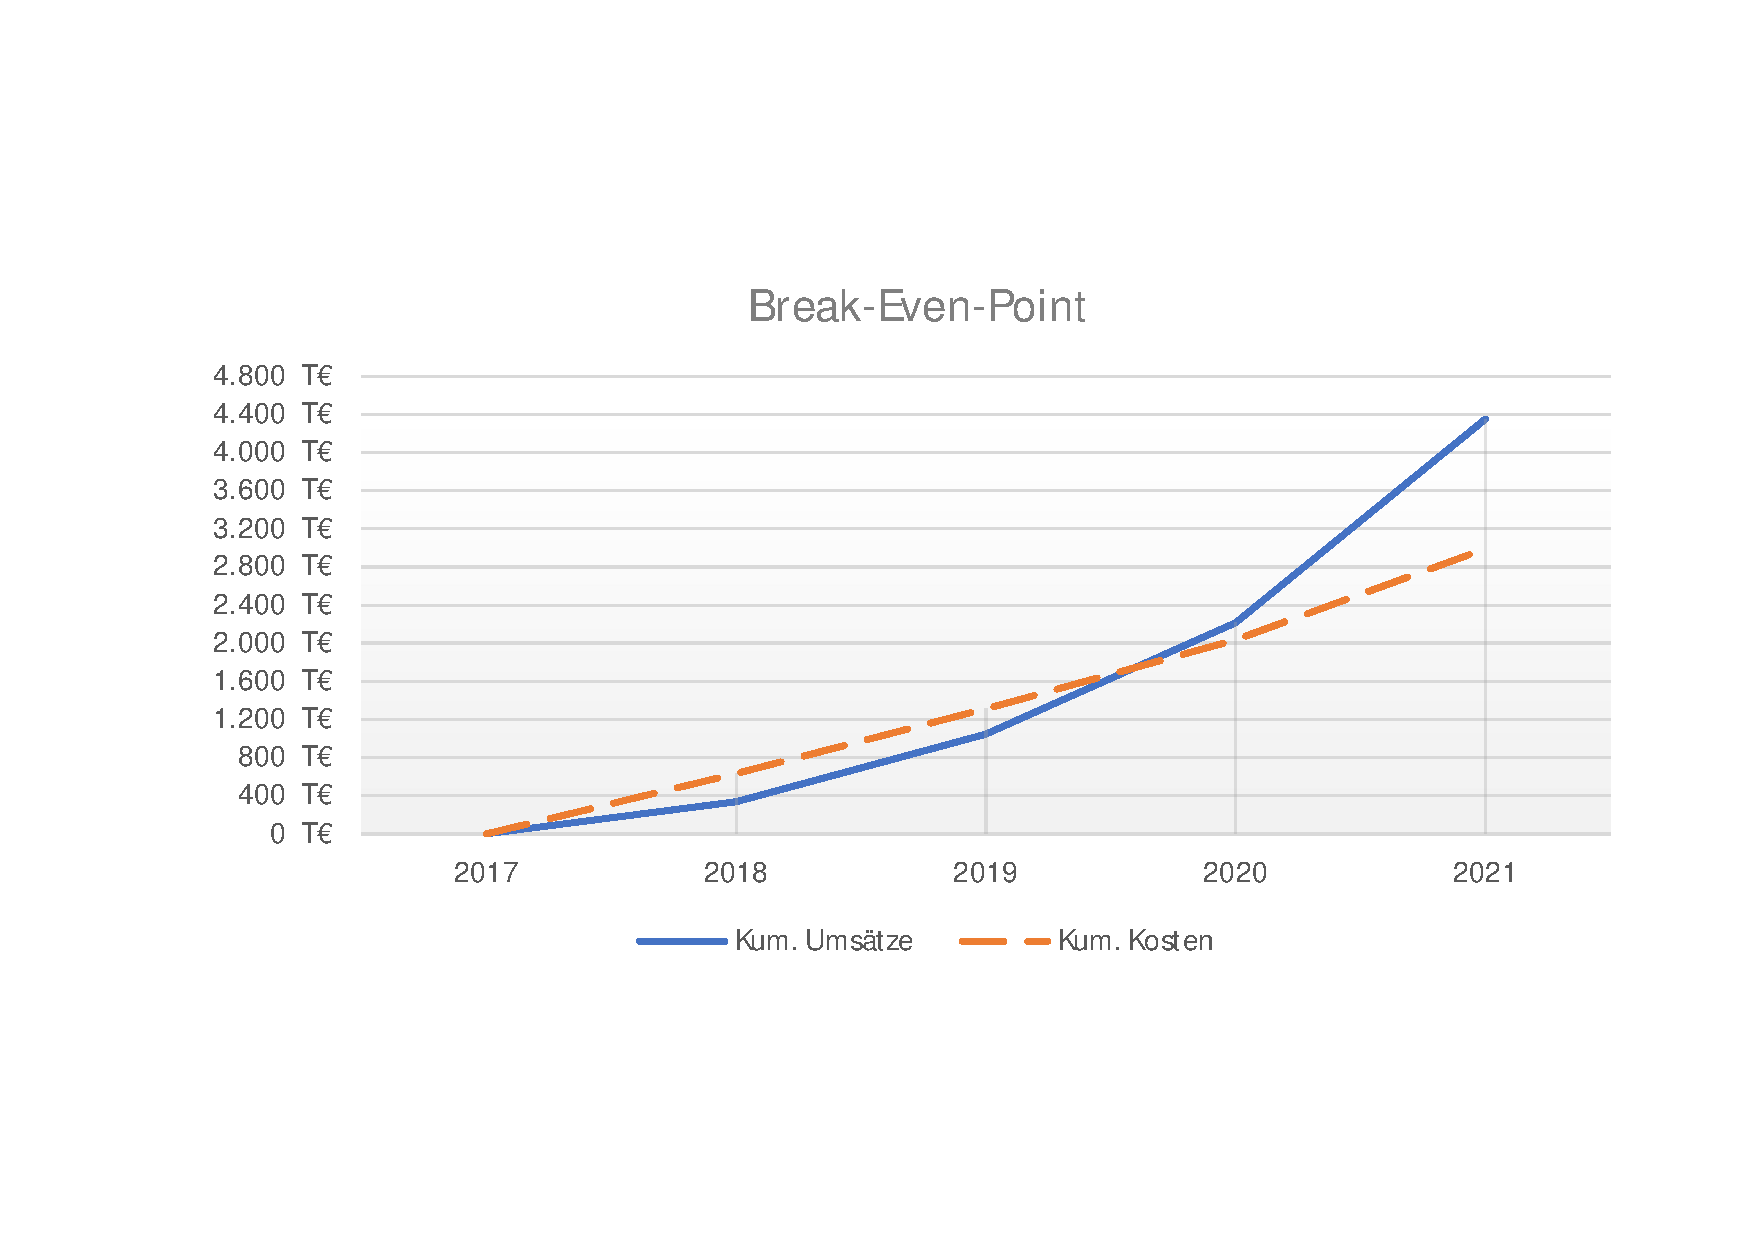
\includegraphics[width=10cm]{BasisSzenario-BEP.pdf}
	\caption{Break-Even-Point im Basis-Szenario}
	\label{fig:BasisSzenario-BEP}
\end{figure}

\subsection{Kapitalbedarf}
Der Kapitalbedarf bis zum BEP beträgt höchstens $220.000$\officialeuro.\\
Um diese Lücke zu schließen, werden folgende Finanzierungsmöglichkeiten geplant:
\begin{itemize}
	\item Einreichung eines Antrags bei der FFG im Basisprogramm zur Förderung von Einzelprojekten.
	\item UBG Gründerfonds
	\item Zusätzliches Eigenkapital
\end{itemize}
Dadurch ergibt sich folgende Finanzierung:\\
\begin{tabular}{l r}
	Kapitalbedarf & $-220.000$\officialeuro \\
	\hline
	FFG Basisprogramm(Projektsumme: $200.000$\officialeuro) & $+100.000$\officialeuro \\
	UBG Gründerfond & $+75.000$\officialeuro \\
	Zusätzliches Eigenkapital & $+45.000$\officialeuro \\
	\bottomrule
\end{tabular}\\
\\
\\Kurzfristige Liquiditätsschwankungen (spätere Zahlungen der Kunden, Projektvorfinanzierung, …) werden mit einem Kontokorrentkredit abgedeckt.

\subsection{Kennzahlen}
\begin{figure}[h]
	\centering
	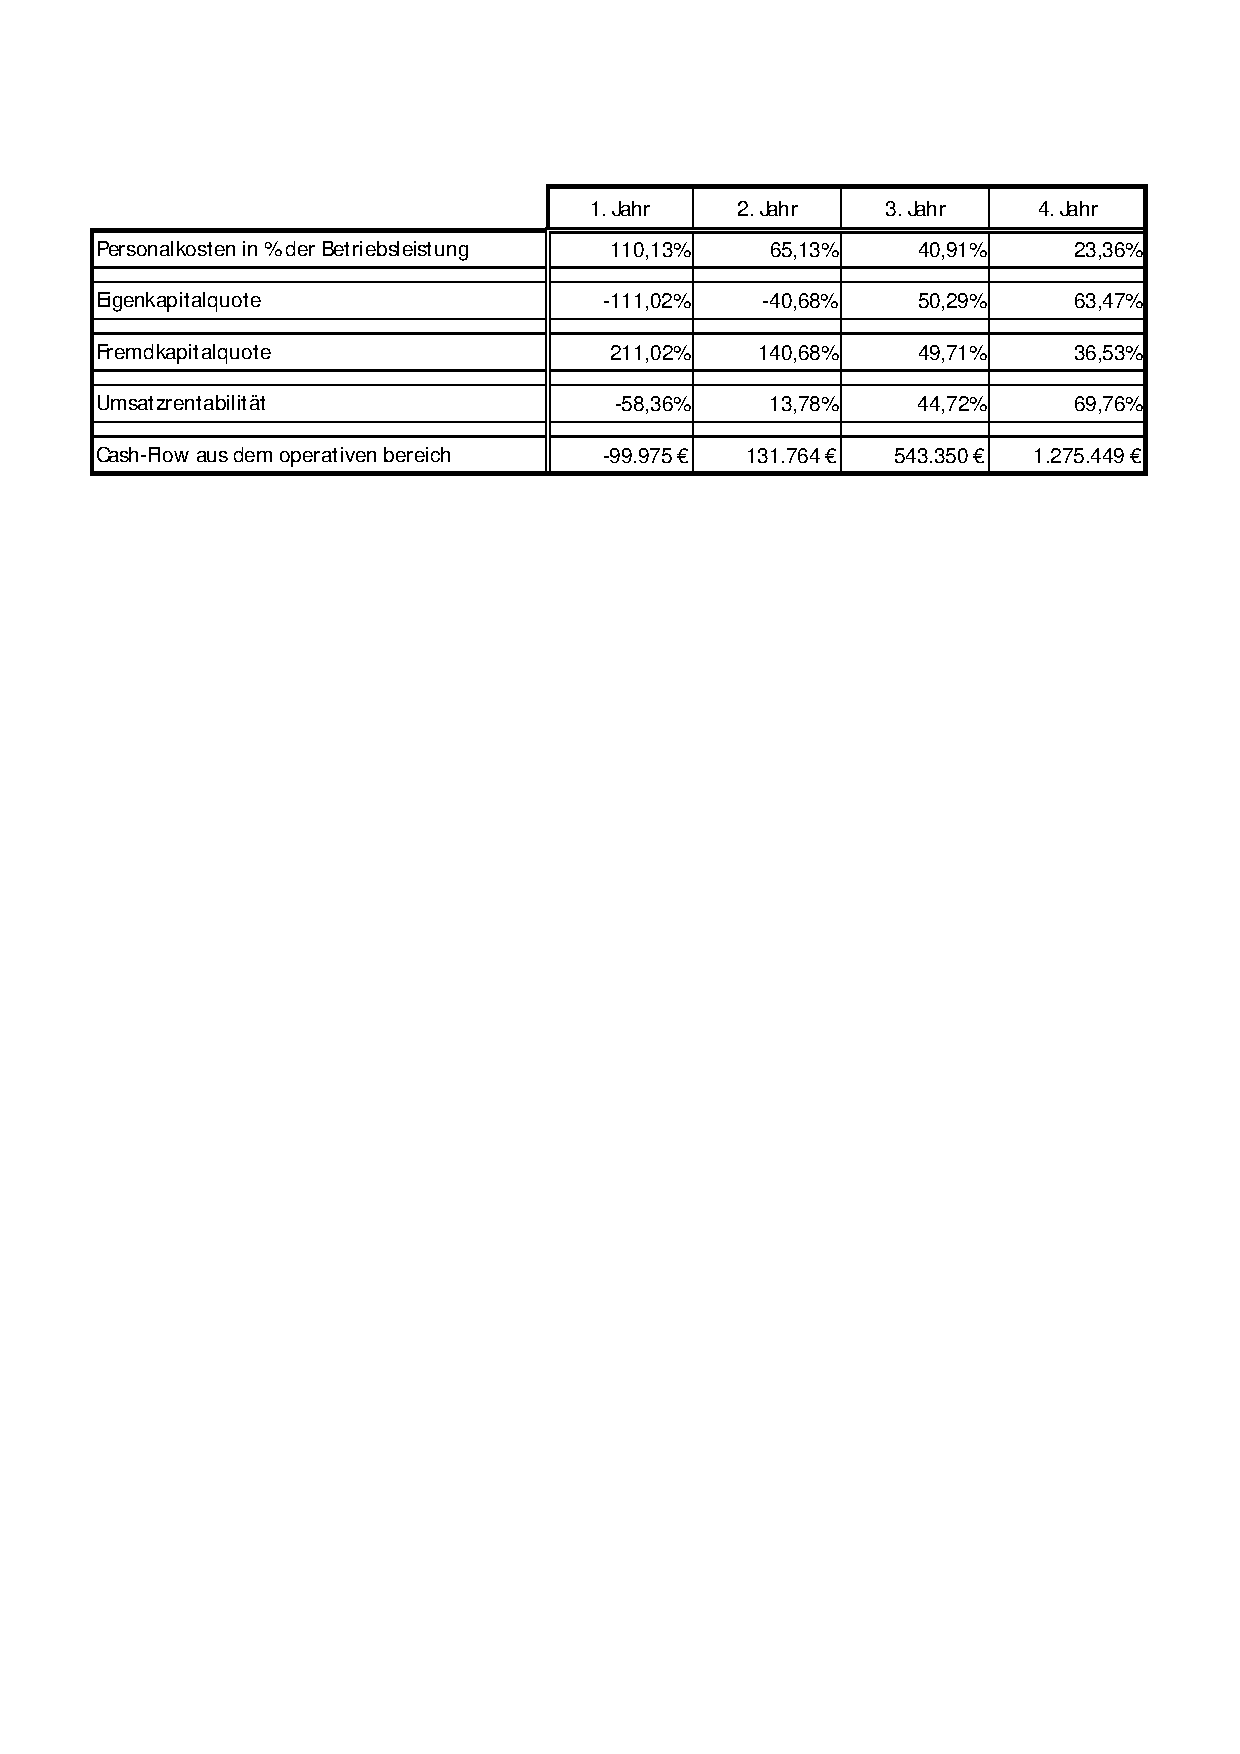
\includegraphics[width=15cm]{BasisSzenario-Kennzahlen.pdf}
	\caption{Kennzahlen im Basis-Szenario}
	\label{fig:BasisSzenario-Kennzahlen}
\end{figure}
\newpage
\subsection{Planbilanz}
\begin{figure}[h]
	\centering
	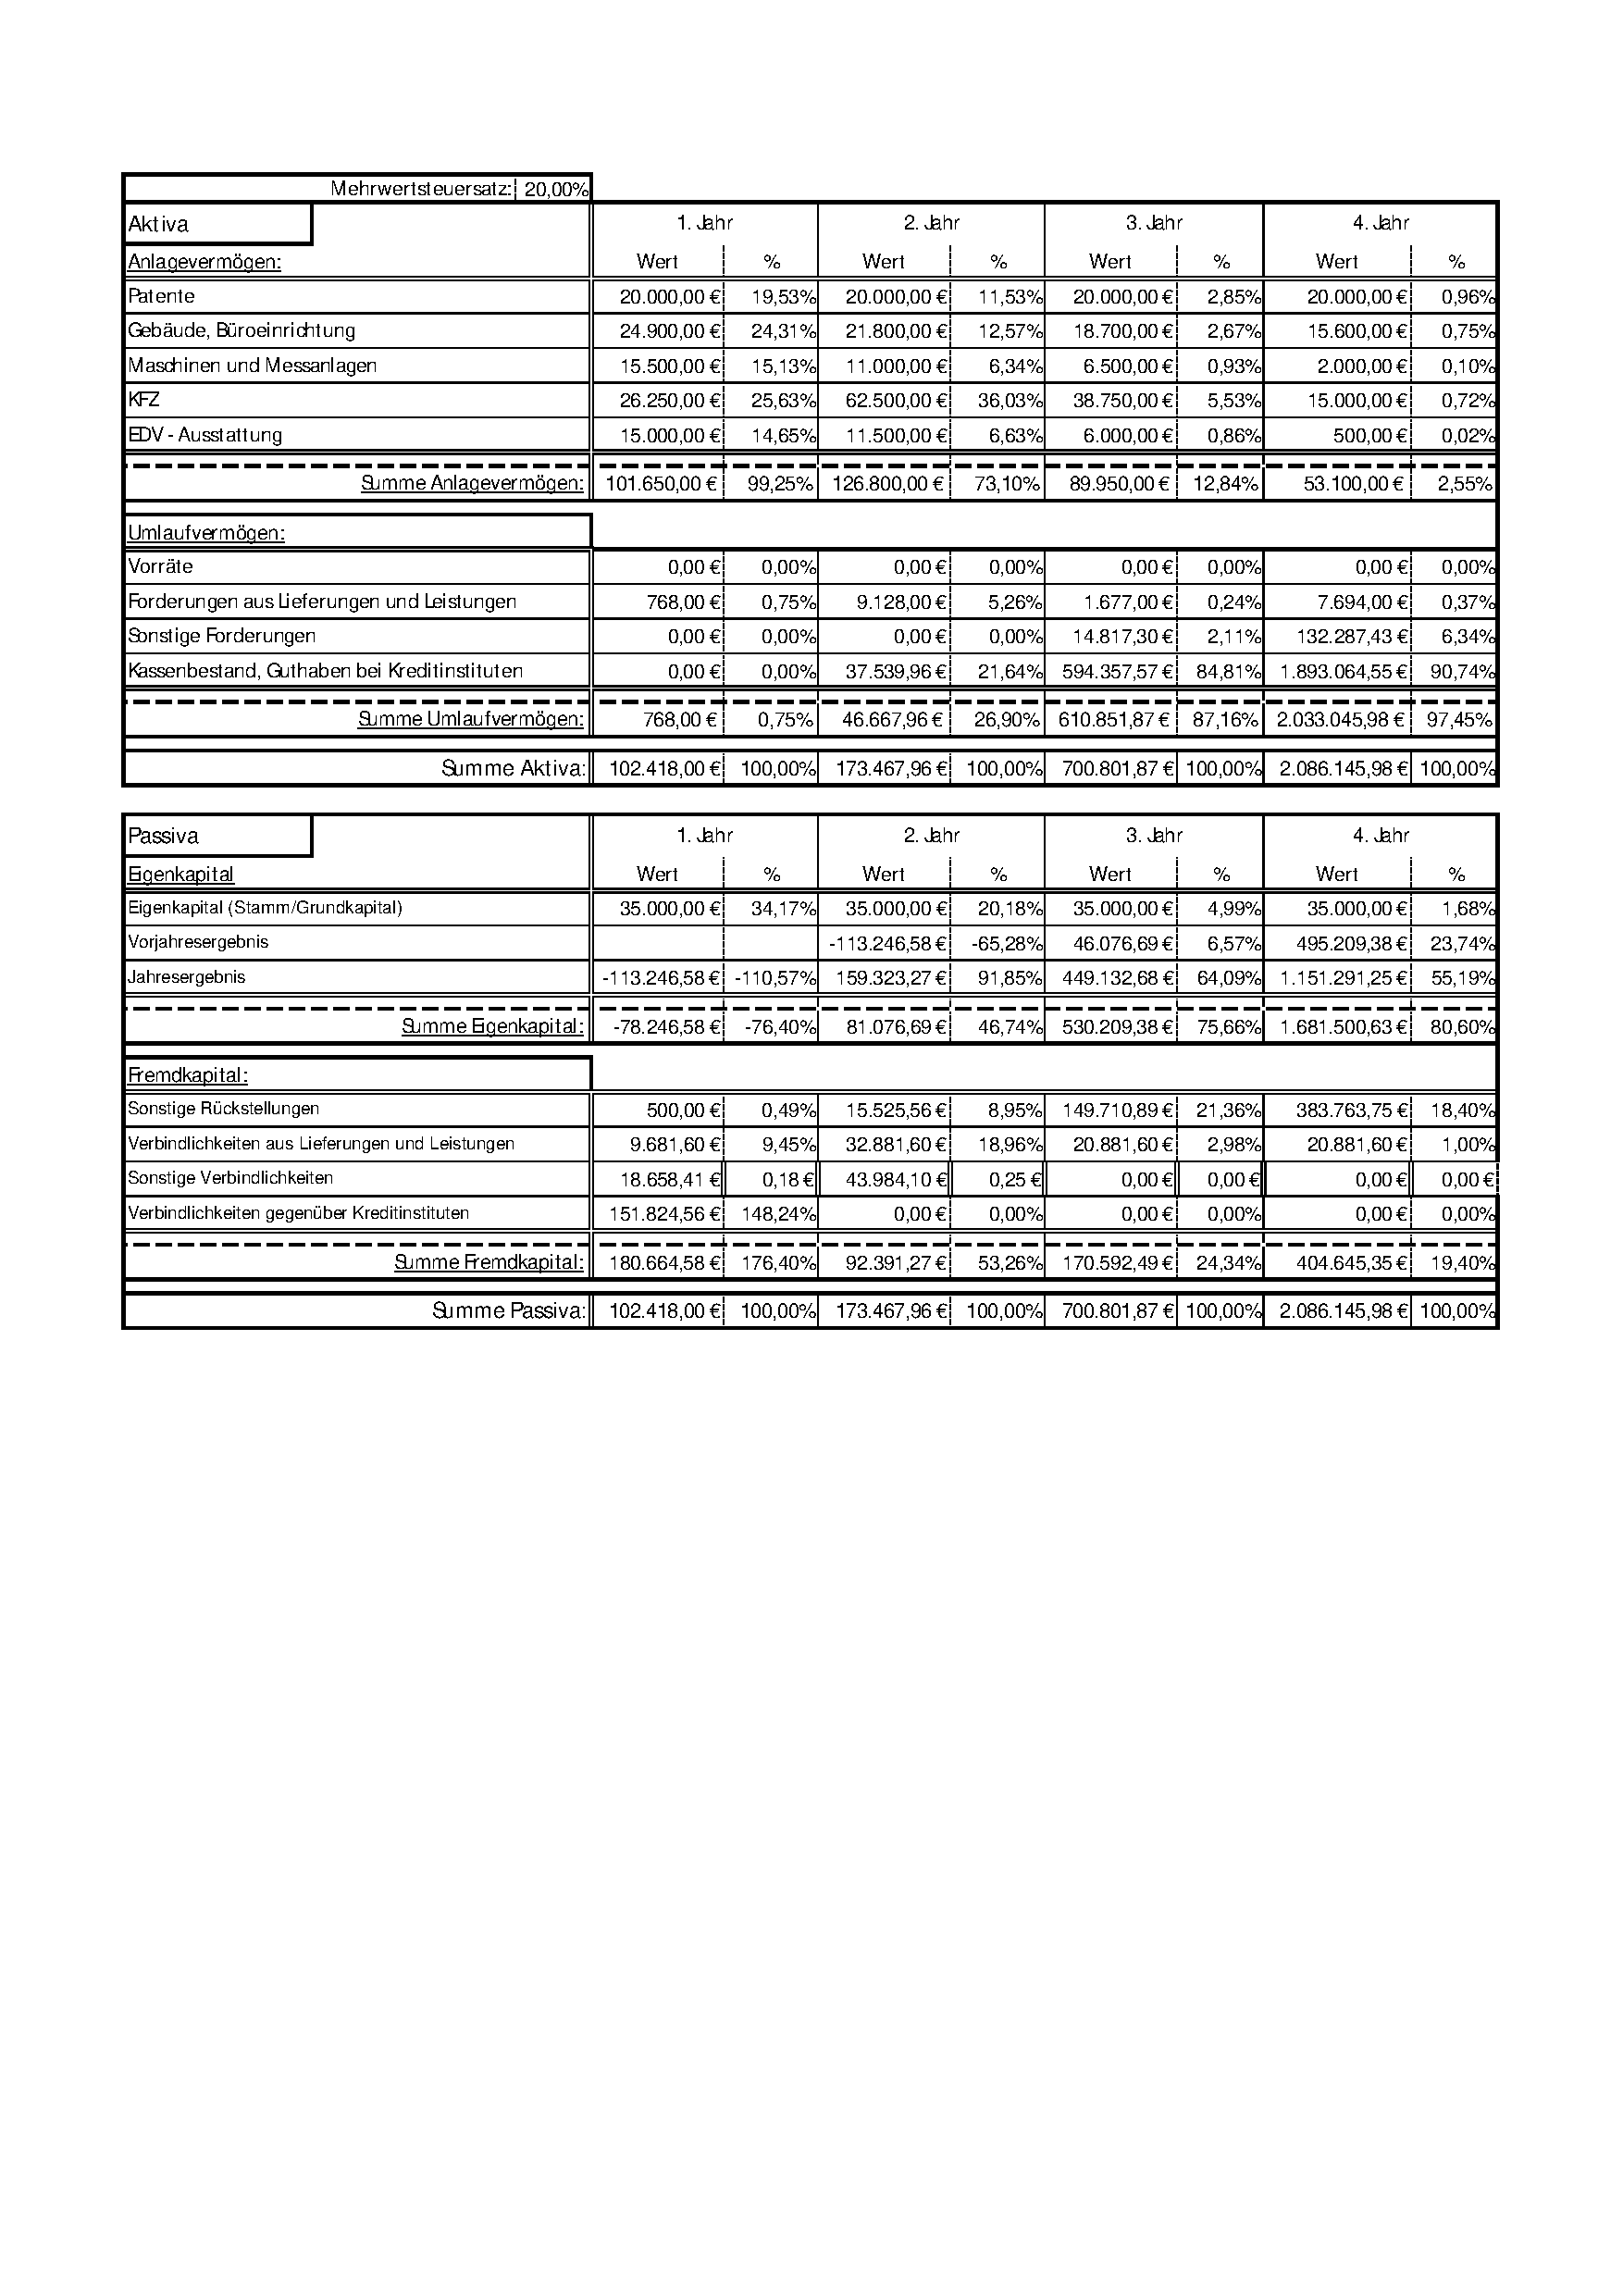
\includegraphics[width=15cm]{BasisSzenario-Planbilanz.pdf}
	\caption{Planbilanz im Basis-Szenario}
	\label{fig:BasisSzenario-Planbilanz}
\end{figure}

\newpage
\subsection{Liquiditätsplan}
\begin{figure}[htp!]
	\centering
	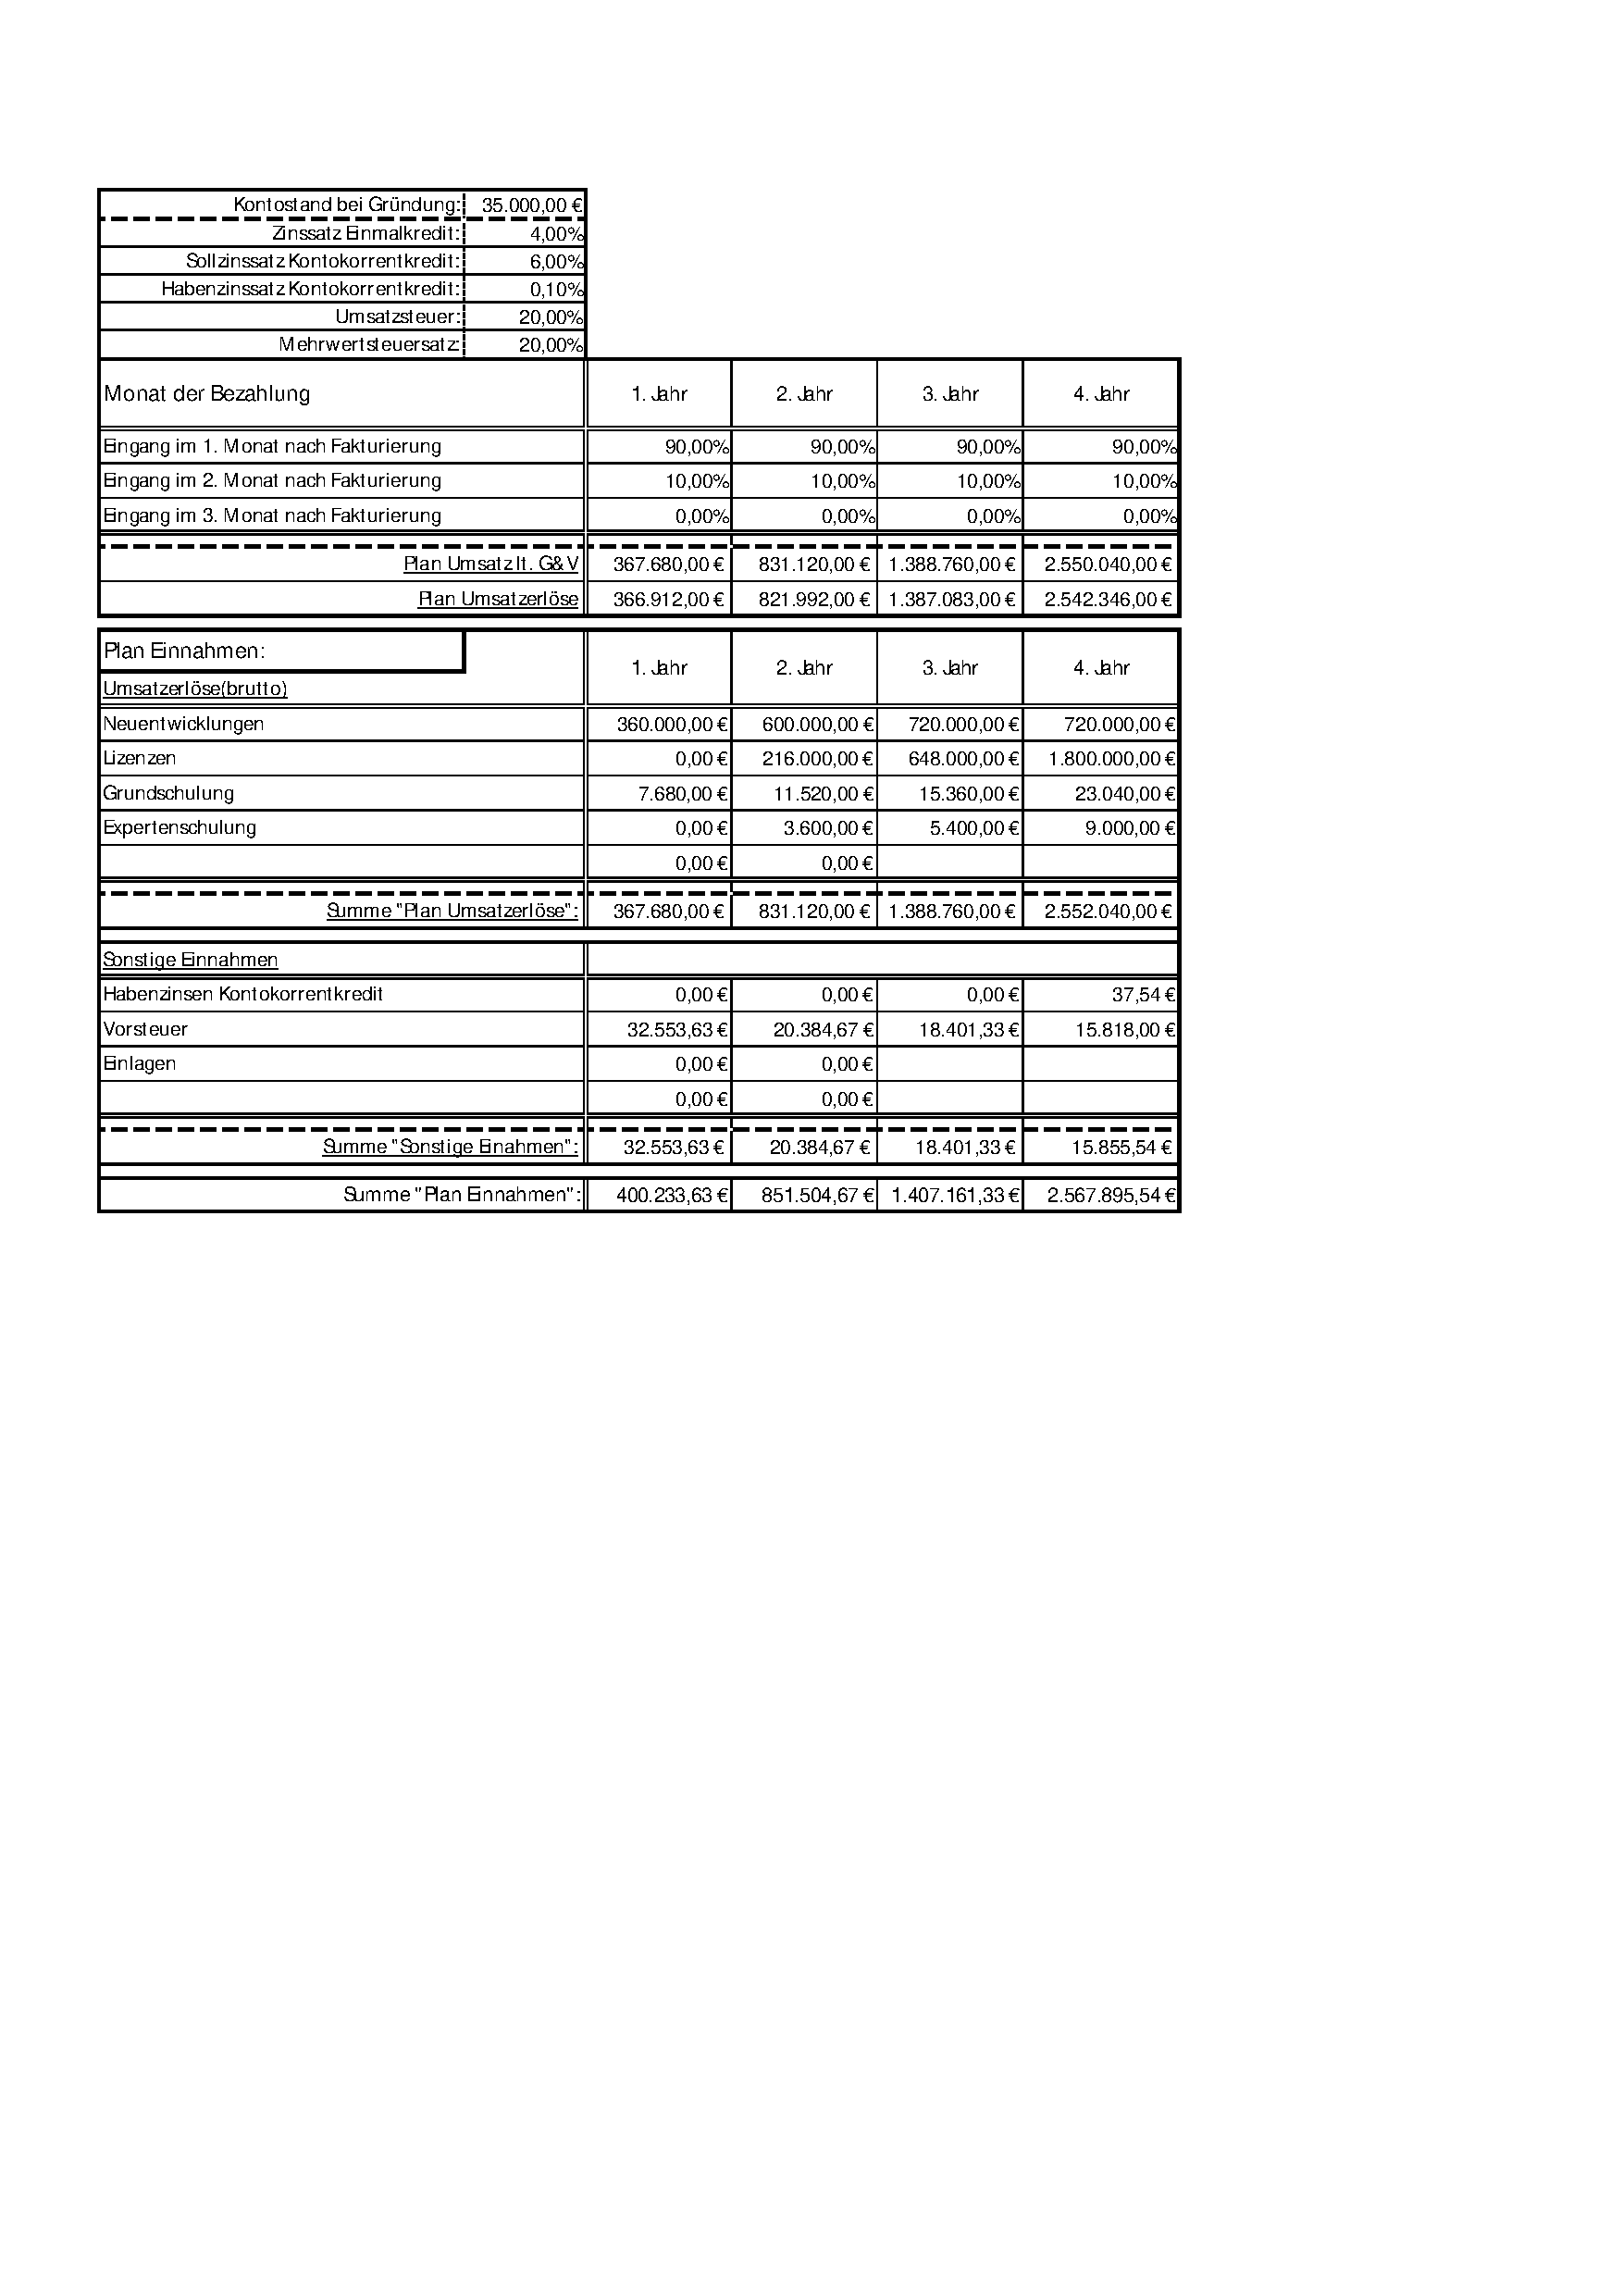
\includegraphics[page=1,width=15cm]{BasisSzenario-Liquiditaet.pdf}
	\label{fig:BasisSzenario-Liquiditaet-1}
\end{figure}
\begin{figure}[htp!]
	\centering
	\includegraphics[page=2,width=15cm]{BasisSzenario-Liquiditaet.pdf}
	\caption{Liquiditätsplan im Basis-Szenario}
	\label{fig:BasisSzenario-Liquiditaet-2}
\end{figure}

\newpage
\subsection{Plan Gewinn- \& Verlustrechnung}
\begin{figure}[htp!]
	\centering
	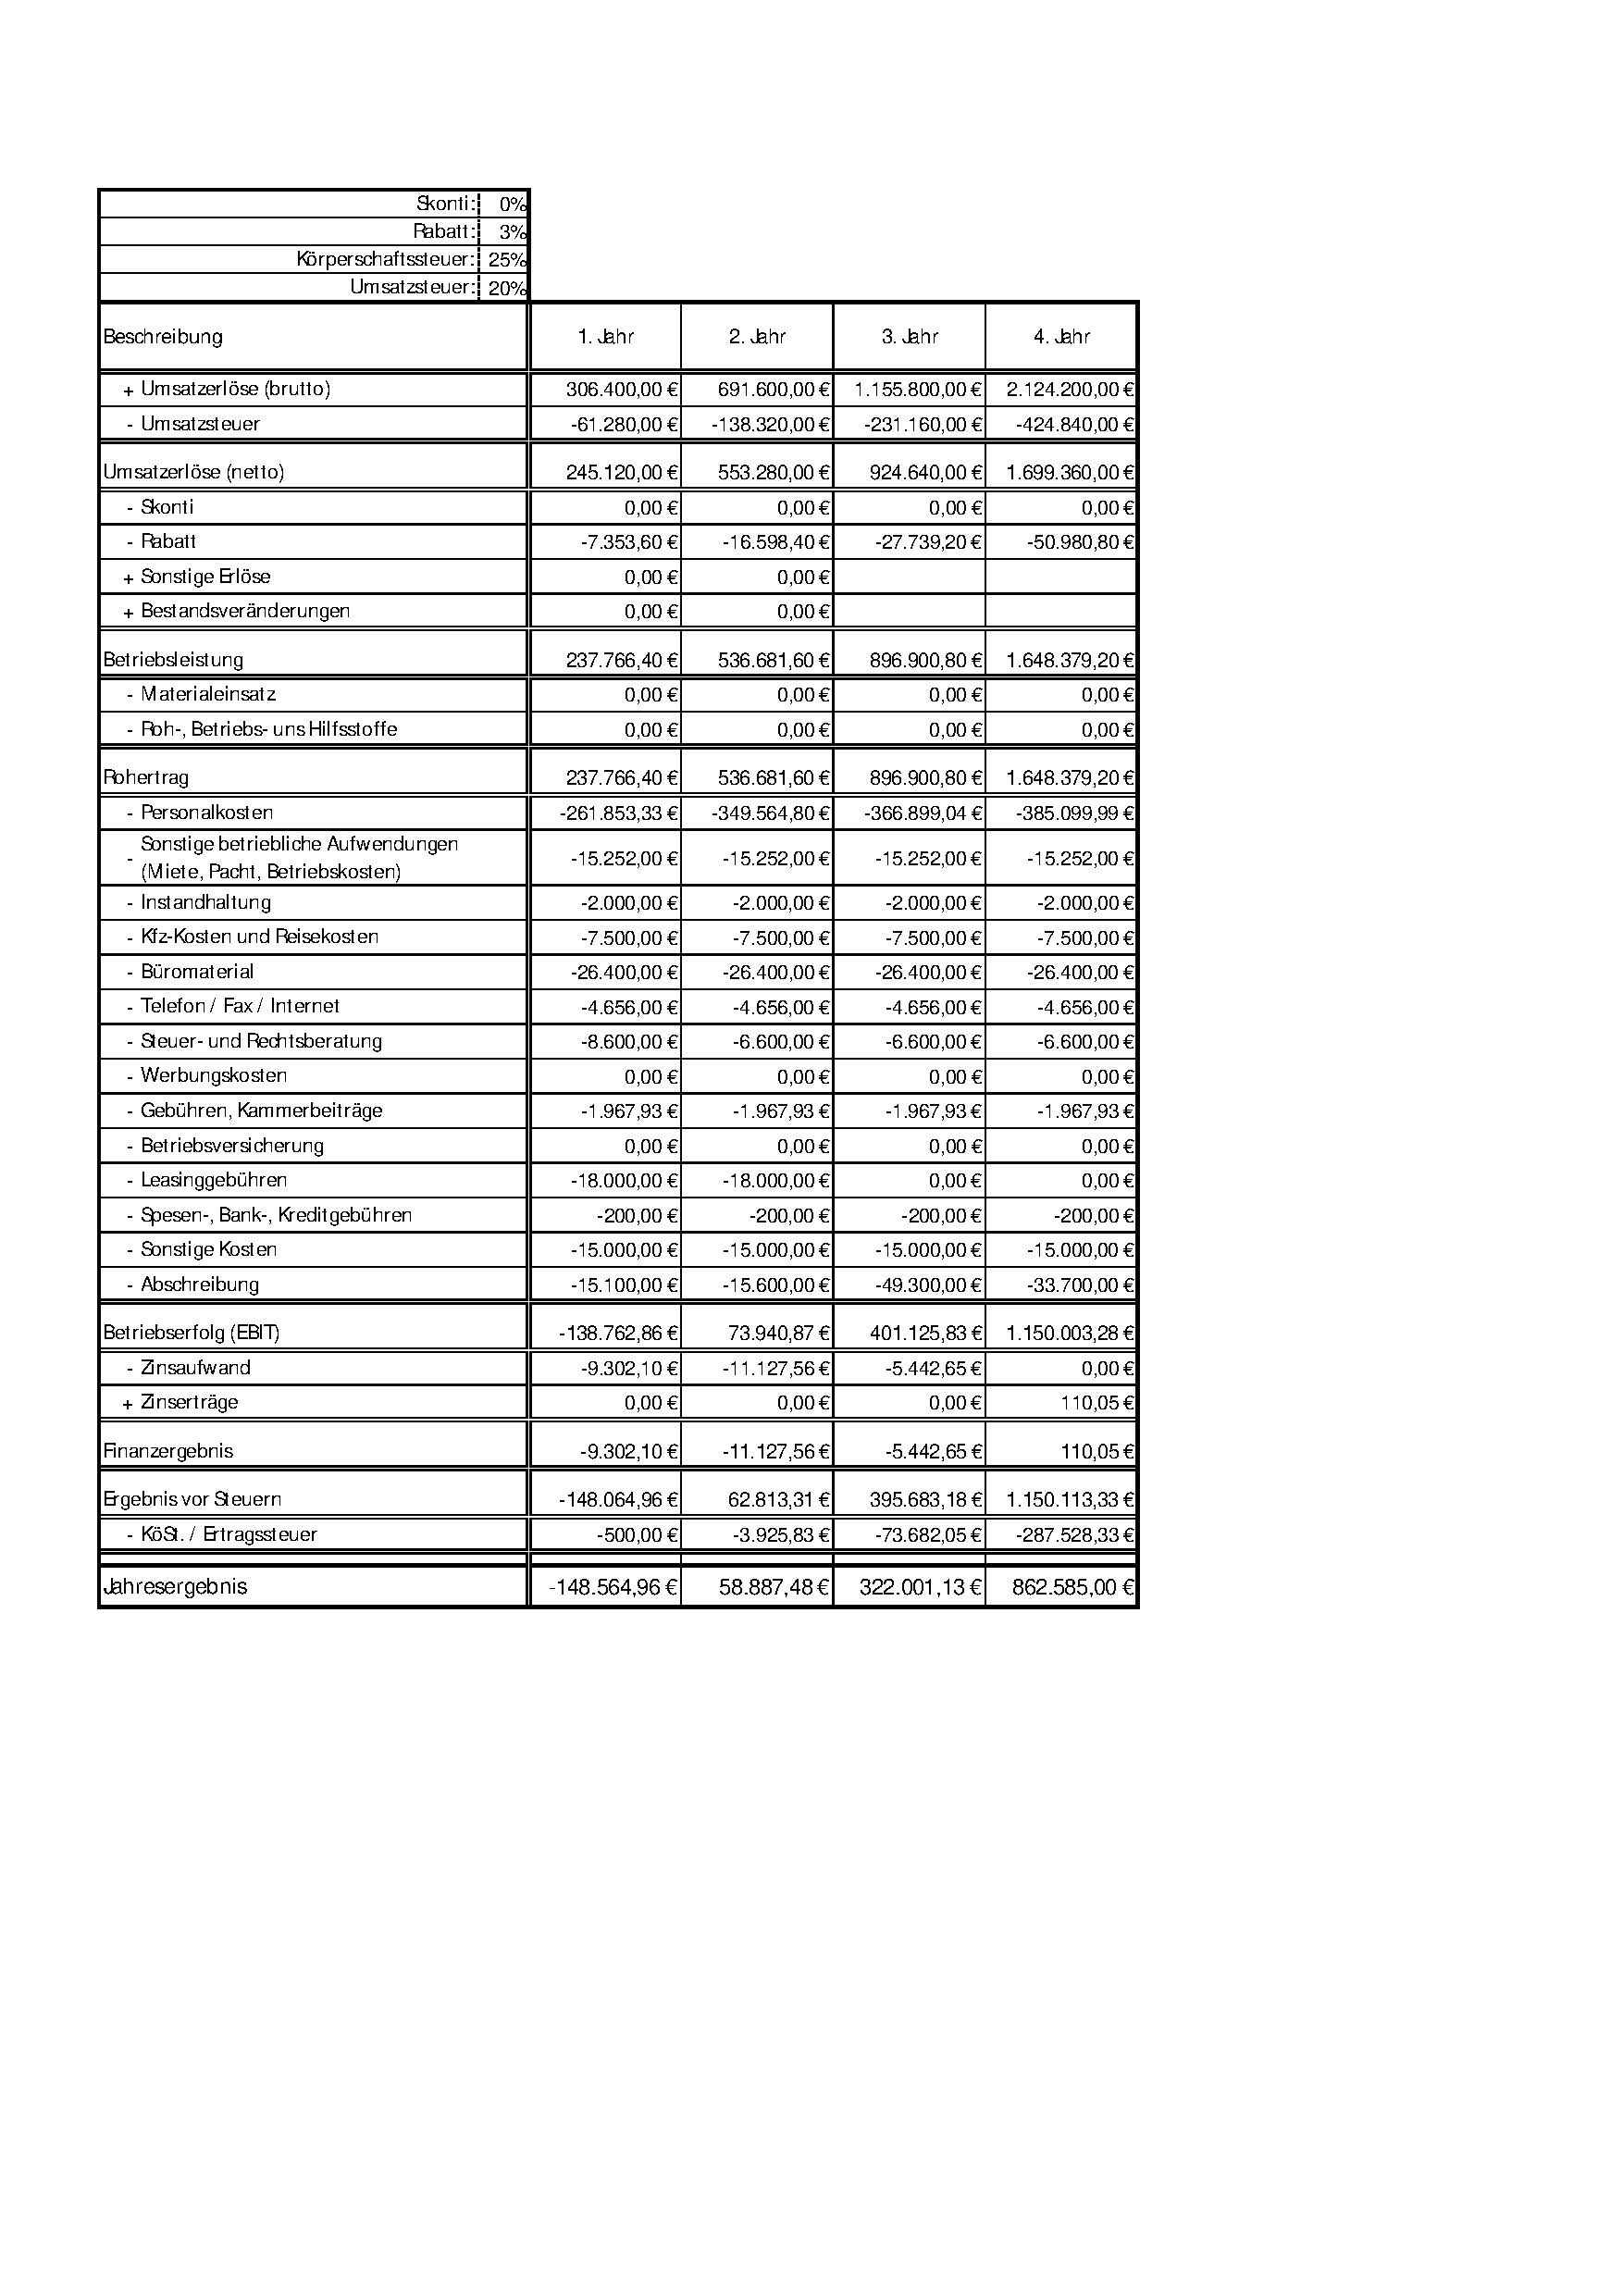
\includegraphics[width=13.3cm]{BasisSzenario-PlanGuV.pdf}
	\caption{Gewinn- \& Verlustrechnung im Basis-Szenario}
	\label{fig:BasisSzenario-GuV}
\end{figure}

\newpage
\subsection{Investition}
\begin{figure}[htp!]
	\centering
	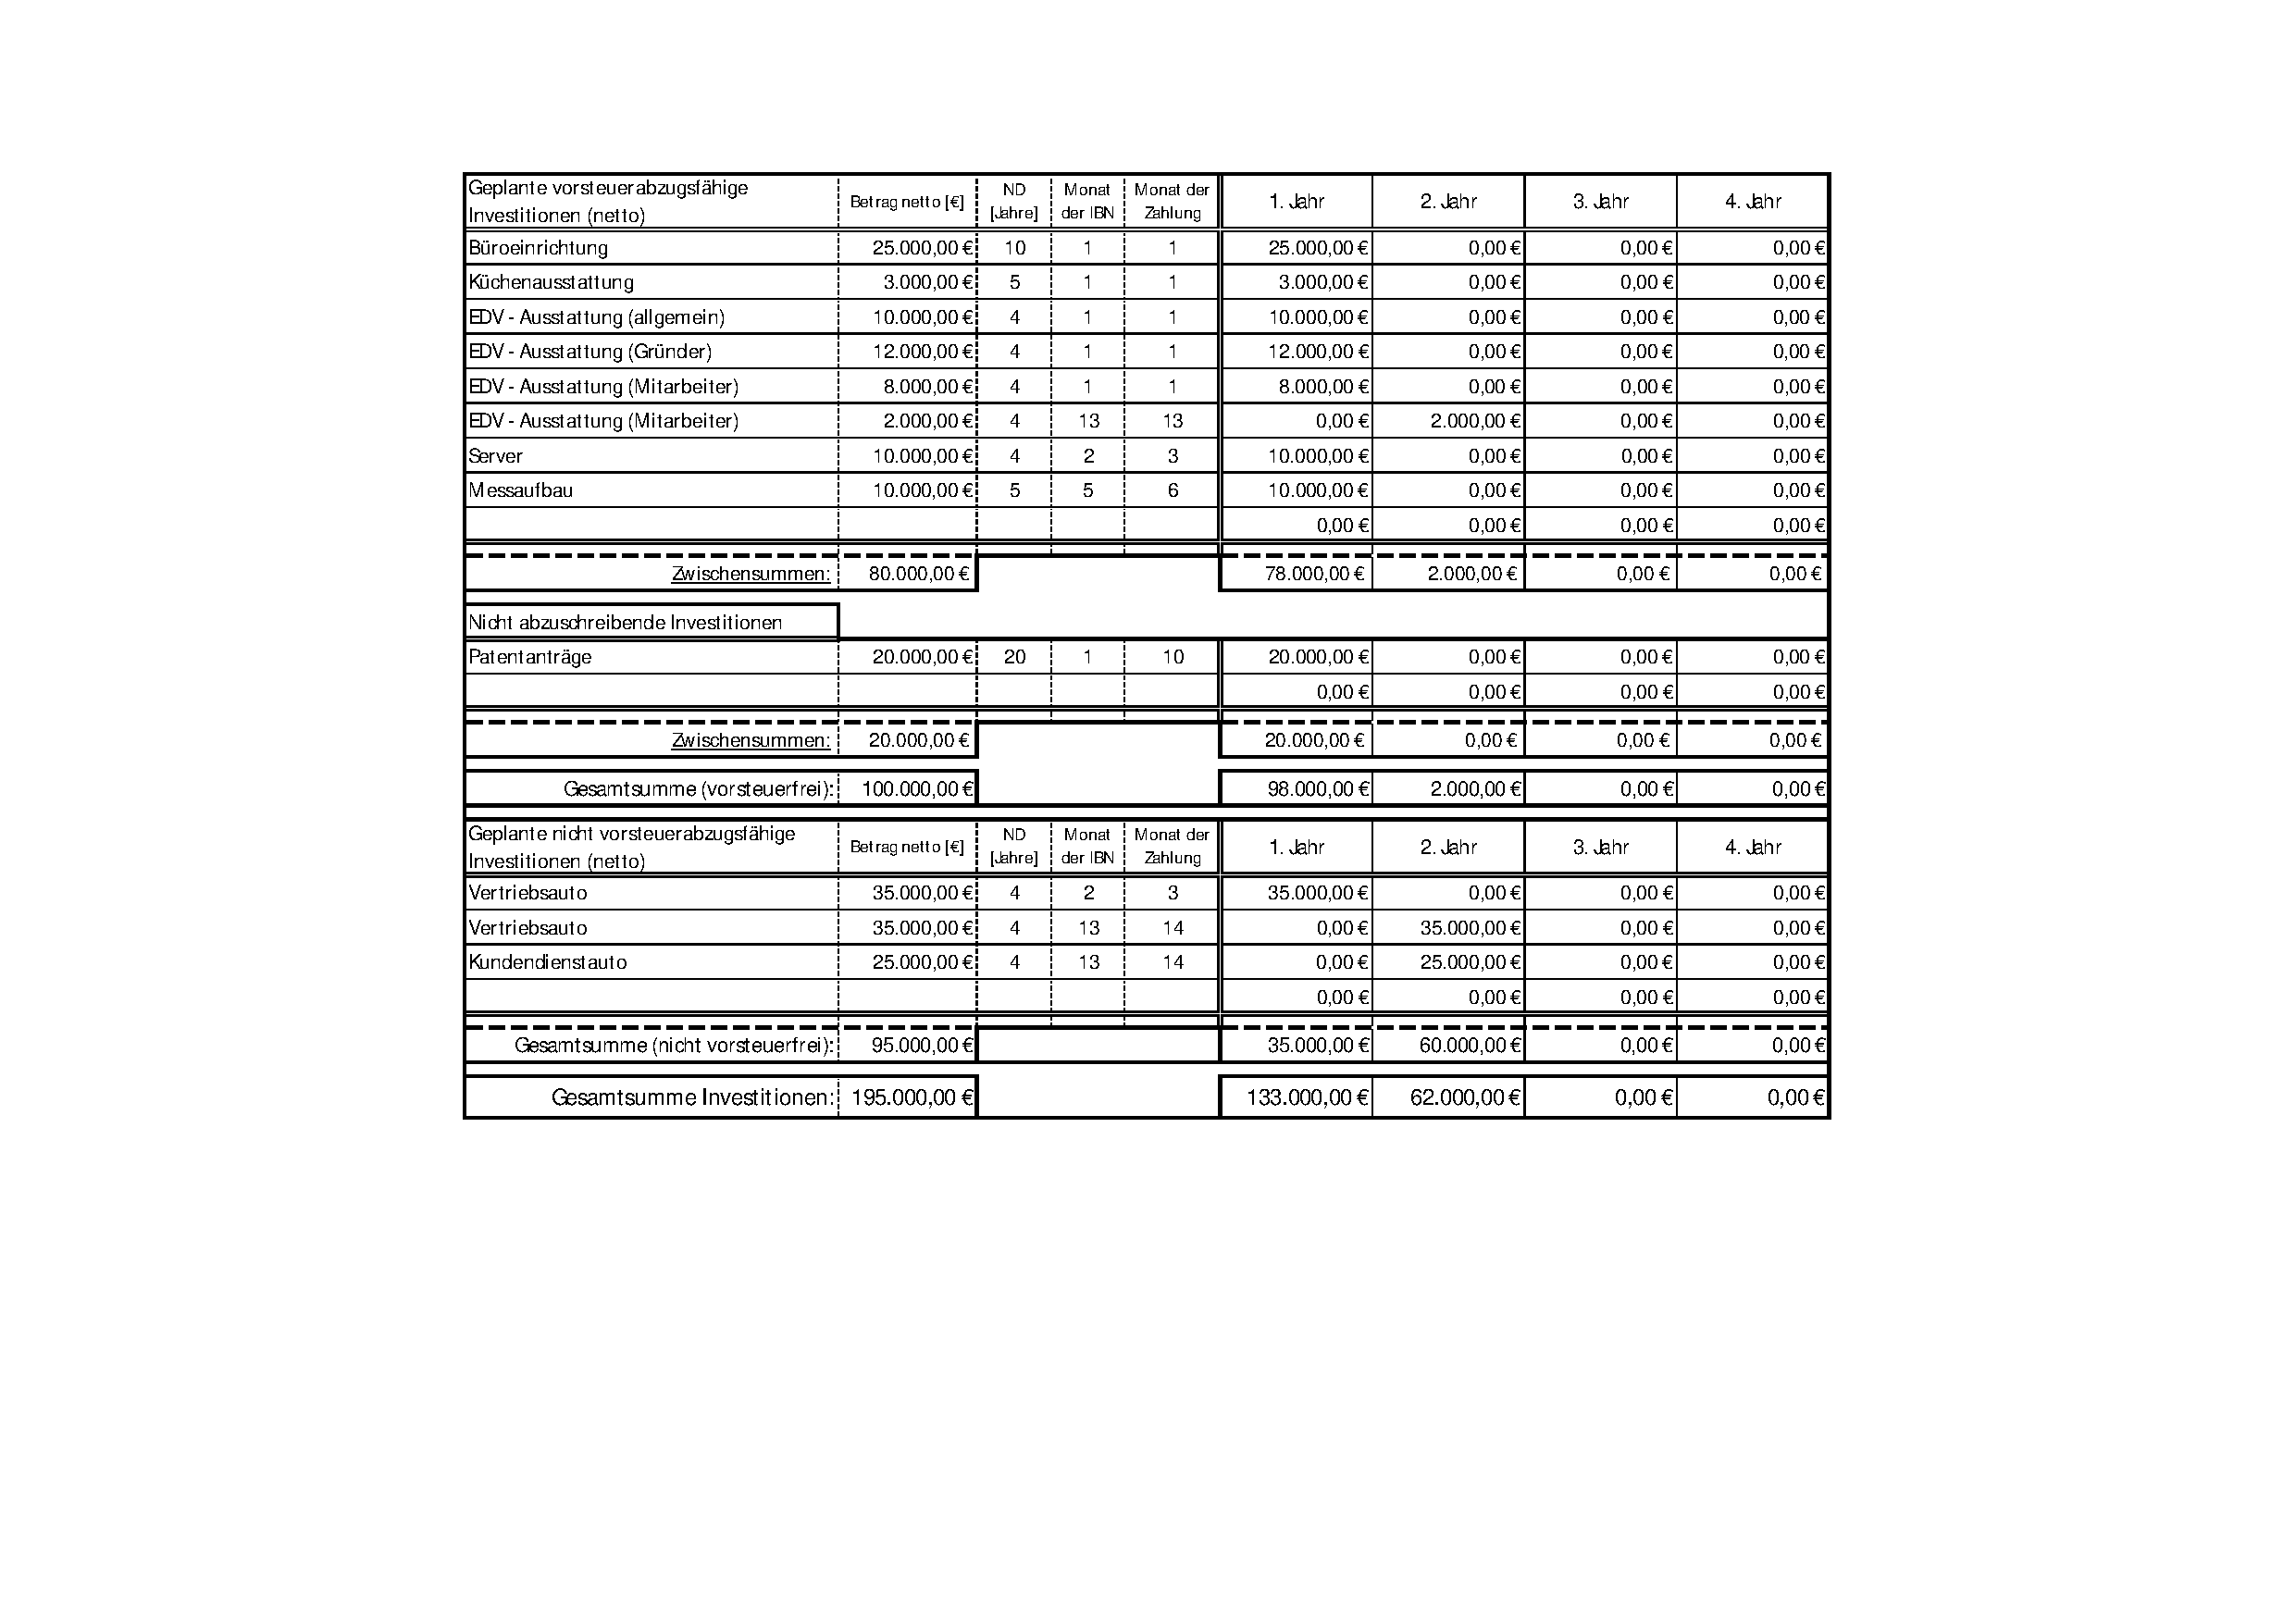
\includegraphics[width=15cm]{BasisSzenario-Investitionen.pdf}
	\caption{Investitionen im Basis-Szenario}
	\label{fig:BasisSzenario-Investitionen}
\end{figure}

\begin{landscape}
	\subsection{Aufwände}
	\begin{figure}[htp!]
		\centering
		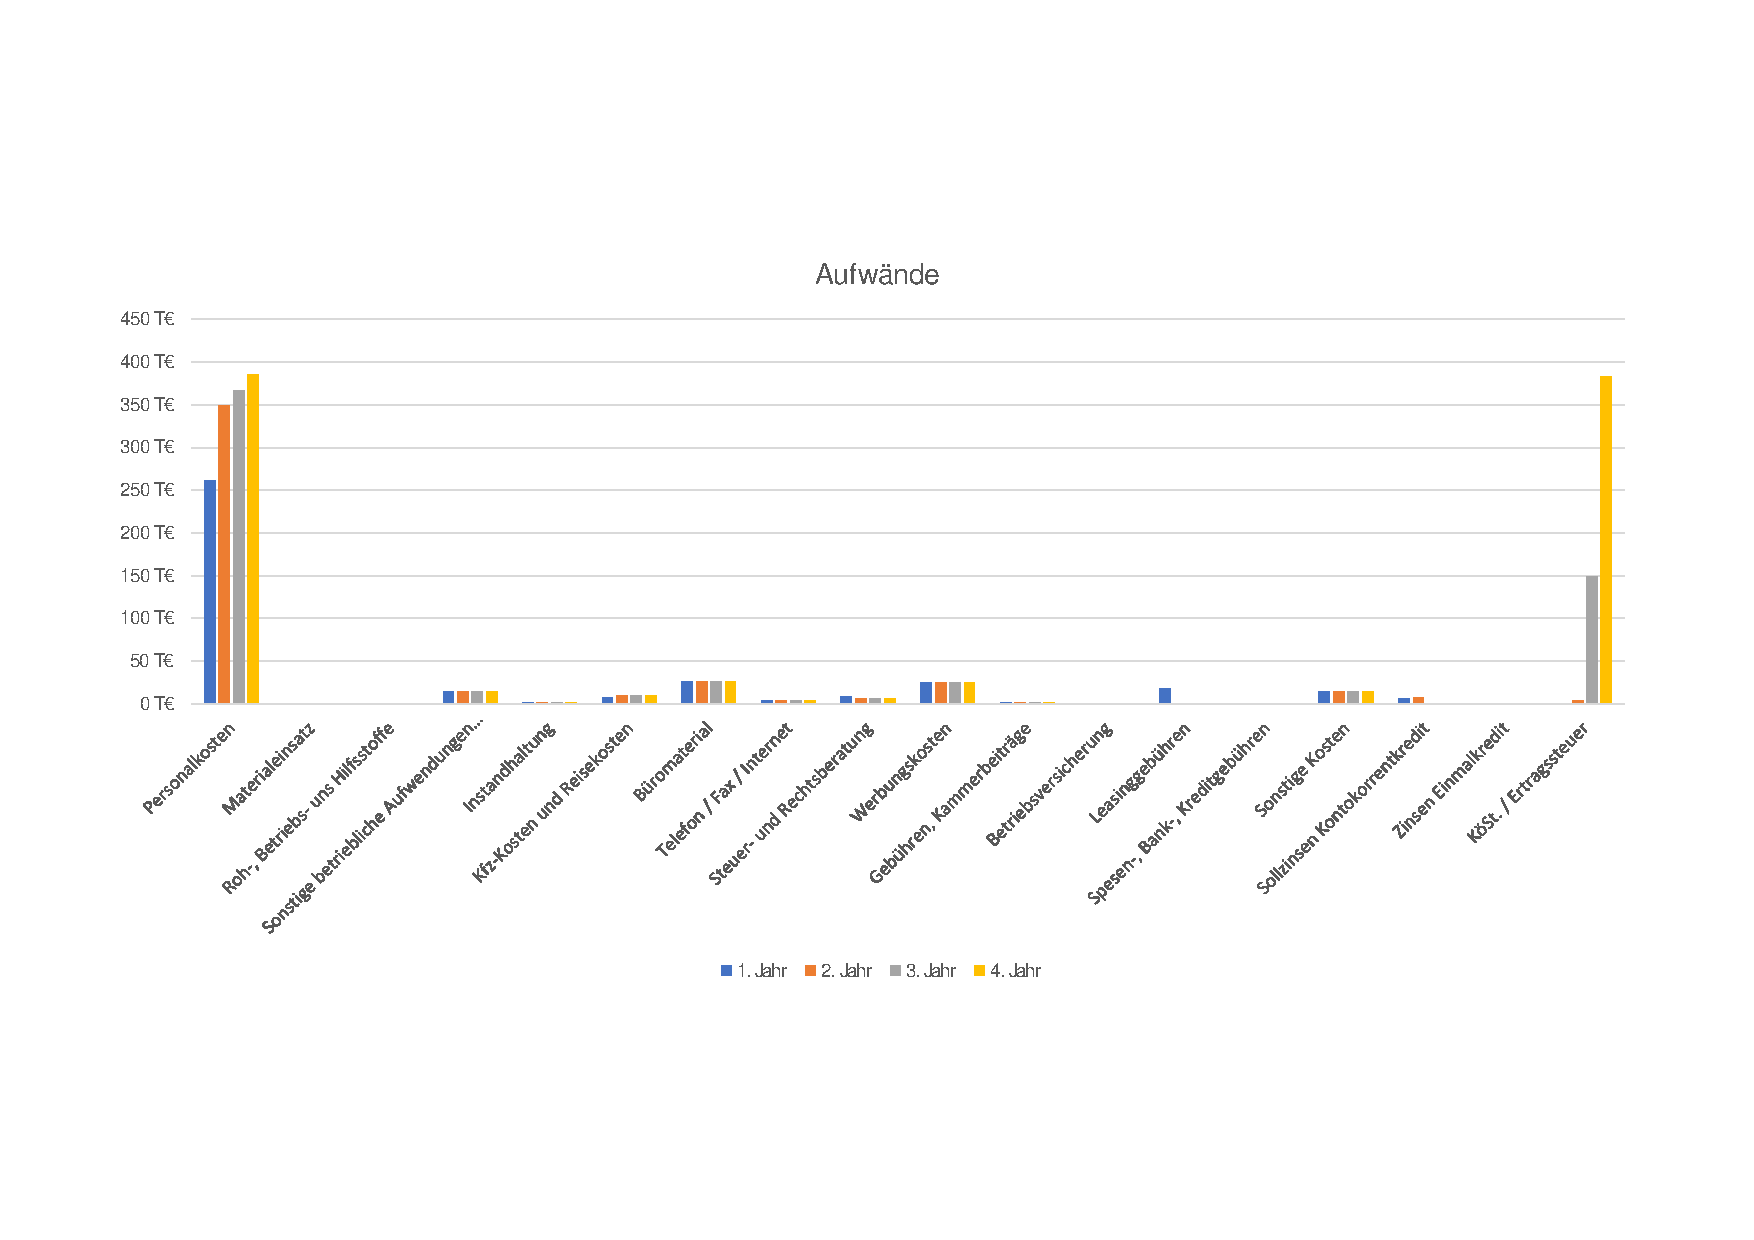
\includegraphics[width=24cm]{BasisSzenario-Aufwaende.pdf}
		\caption{Aufwände im Basis-Szenario}
		\label{fig:BasisSzenario-Aufwaende}
	\end{figure}
\end{landscape}

\newpage
\section{Best-Case-Szenario}
Für das Basis-Scenario wurden folgende Annahmen getroffen:
\begin{itemize}
	\item Es werden in den folgenden 4 Jahren 30 Neuentwicklungen in Auftrag gegeben (Aufteilung:~4/6/8/12).
	\item Die Lizenzvergabe verteilt sich wie folgt:\newline (Angaben in Prozent vom weltweitem Verkauf von Industrierobotern)
	\begin{itemize}
		\item 1. Jahr: $0,00$\% (0 Roboter)
		\item 2. Jahr: $0,05$\% (~200 Roboter)
		\item 3. Jahr: $0,10$\% (~400 Roboter)
		\item 4. Jahr: $1,00$\% (~4000 Roboter)
	\end{itemize}
	\item Die durchschnittlichen Lizenzkosten betragen $1.500,00$ \officialeuro.
	\item Es wird mit 120 Schulungsteilnehmer innerhalb der nächsten 4 Jahren gerechnet (Aufteilung:~8/24/36/52). Hauptsächlich werden Grundschulung in Anspruch genommen. Daher betragen die durchschnittlichen Schulungskosten $1.100,00$~\officialeuro.
\end{itemize}

\section{Worst-Case-Szenario}
Für das Basis-Scenario wurden folgende Annahmen getroffen:
\begin{itemize}
	\item Es werden in den folgenden 4 Jahren 10 Neuentwicklungen in Auftrag gegeben (Aufteilung:~1/2/3/4).
	\item Die Lizenzvergabe verteilt sich wie folgt:\newline (Angaben in Prozent vom weltweitem Verkauf von Industrierobotern)
	\begin{itemize}
		\item 1. Jahr: $0,00$\% (0 Roboter)
		\item 2. Jahr: $0,01$\% (~40 Roboter)
		\item 3. Jahr: $0,03$\% (~120 Roboter)
		\item 4. Jahr: $0,06$\% (~240 Roboter)
	\end{itemize}
	\item Die durchschnittlichen Lizenzkosten betragen $1.500,00$ \officialeuro.
	\item Es wird mit 25 Schulungsteilnehmer innerhalb der nächsten 4 Jahren gerechnet (Aufteilung:~3/5/7/10). Hauptsächlich werden Grundschulung in Anspruch genommen. Daher betragen die durchschnittlichen Schulungskosten $900,00$~\officialeuro.
\end{itemize}